\documentclass[dvipdfmx, dvipsnames]{beamer}
\usetheme[secheader]{Boadilla}
% \usepackage{beamerthemesplit} // Activate for custom appearanced
%\setbeamertemplate{caption}[numbered]
\usefonttheme[onlymath]{serif} %数式をゴシックにしない
\setbeamertemplate{blocks}[rounded] % Blockの影を消す
\useinnertheme{circles} % 箇条書きをシンプルに
\setbeamertemplate{navigation symbols}{} % ナビゲーションシンボルを消す
\setbeamertemplate{footline}[frame number] % フッターはスライド番号のみ
\setbeamercolor{page number in head/foot}{fg=black}
% \usepackage{beamerthemesplit} // Activate for custom appearance
\setlength{\parindent}{1em}  %段落字下げ
\renewcommand{\figurename}{Fig}
\renewcommand{\tablename}{Tab}
\usepackage[caption=false]{subfig}
\usepackage{tikz}  
\usetikzlibrary{decorations.pathreplacing,calligraphy}
\usetikzlibrary{angles,quotes} % for pic
\setbeamerfont{itemize/enumerate subbody}{size=\normalsize}
%
%\setbeamertemplate{itemize subitem}{\normalsize\raise1.25pt\hbox{\donotcoloroutermaths$\blacktriangleright$}}  %to set the symbol size
\usetikzlibrary{shapes,positioning}
\usepackage{xcolor}


\def\mathunderline#1#2{\color{#1}\underline{{\color{black}#2}}\color{black}}

%def symbol
\newcommand{\normal}{\mathcal{N}}
\newcommand{\exponential}{\mathcal{E}}
\newcommand{\truncnorm}{\mathcal{TN}}
\newcommand{\gam}{\mathcal{G}}
\newcommand{\C}{C}
\newcommand{\one}{1\!\!1}

\title{テンソル同時分解の拡張による\\オミクスデータの統合}
\date{2023年6月3日}
\author {阿部興\footnote{東京医科歯科大学難治疾患研究所} ・島村徹平\footnote{名古屋大学医学系研究科・東京医科歯科大学難治疾患研究所}}

\begin{document}
\frame{
\titlepage
}

\renewcommand*{\thefootnote}{\fnsymbol{footnote}}
\setcounter{footnote}{0} 

\section{背景}
\frame{
\frametitle{動機:分析対象}
\begin{figure}
 \begin{tikzpicture}
\node[draw, rounded corners, fill=gray!10](dna) at (0,0){
\includegraphics[width=.05\textwidth]{img/dna.png}DNA};
\node[draw, rounded corners, fill=gray!10, right = of dna, xshift = +15pt](rna){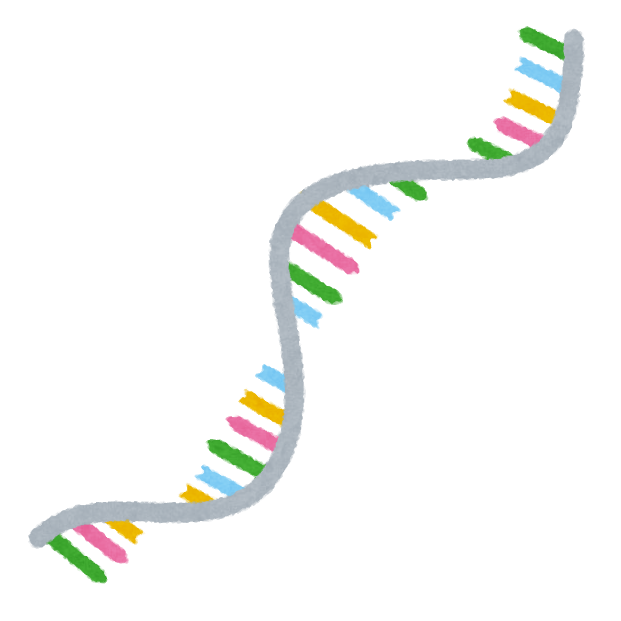
\includegraphics[width=.05\textwidth]{img/body_rna.png}RNA};
\node[draw, rounded corners, fill=gray!10, right = of rna, xshift = +15pt](protein){
\includegraphics[width=.05\textwidth]{img/kagaku_bunshi.png}protein};
\node[draw, rounded corners, fill=gray!10, right = of protein](phenotype) {
\includegraphics[width=.05\textwidth]{img/nut_renzumame.png}phenotype};
%path
\path[draw, ->, darkgray](dna)--(rna) node[midway, below, yshift = -2pt]{転写};
\path[draw, ->,darkgray](rna)--(protein) node[midway, below, yshift = -2pt]{翻訳};
\path[draw, dashed, ->, darkgray](protein)--(phenotype);
%omics
\node[below= of dna](genomics){genomics};
\node[below= of rna](transcriptomics){transcriptomics};
\node[below= of protein](proteomics){proteomics};

\node[above= of dna, yshift=-5ex]{\textcolor{darkgray}{モダリティ}};

\path[draw, RoyalBlue](dna)--(genomics);
\path[draw, RedOrange](rna)--(transcriptomics);
\path[draw, RedOrange](proteomics)--(protein);

\path[draw, RedOrange, dashed](genomics.north west)--(proteomics.north east);
\path[draw, RedOrange, dashed](genomics.south west)--(proteomics.south east);
\path[draw, RedOrange, dashed](genomics.north west)--(genomics.south west);
\path[draw, RedOrange, dashed](proteomics.north east)--(proteomics.east)node[right](omics){-omics};
\end{tikzpicture}
%\caption{}
\end{figure}

オミクス(omics)データを統合して分析したい

\begin{itemize}
\item[] \structure{積極的理由:}データを補い合い普遍的な特徴を抽出
\item[] \structure{消極的理由:}対応のあるサンプルなので非独立
\end{itemize}
}
\frame{
\frametitle{課題:データ統合}
\begin{figure}
 \begin{tikzpicture}
\node[draw, fill=gray!10, text height=1.25ex, text width=8.0ex](mouse) at (0,0){   };
\node[draw, fill=gray!10, right = of mouse, text height=1.25ex, text width=8.0ex](lemur){};
\node[draw,  right = of lemur, text height=1.25ex, text width=8.0ex, align=center](human){?};

\node[above = of mouse, yshift = -25pt] (labmouse){マウス};
\node[above = of lemur, yshift = -25pt](lablemur){サル};
\node[above = of human, yshift = -25pt](labhuman){ヒト};

\path[draw,->, thick](mouse)--(lemur);
\path[draw,->, thick](lemur)--(human);

\node[left = of mouse, xshift = 20pt] (labA){drug A};

\node[draw, fill=gray!10, text height=1.25ex, text width=8.0ex, below=of mouse](mouse2){};
\node[draw, fill=gray!10, right = of mouse2, text height=1.25ex, text width=8.0ex](lemur2){};
\node[draw,  right = of lemur2, text height=1.25ex, text width=8.0ex, align=center](human2){?};

\node[draw, fill=gray!10, text height=1.25ex, text width=8.0ex, below=of mouse2, yshift = 3ex](mouse3){};
\node[draw, right = of mouse3, text height=1.25ex, text width=8.0ex, align=center](lemur3){?};
\node[draw, fill=gray!10, right = of lemur3, text height=1.25ex, text width=8.0ex, align=center](human3){};

\node[draw,  fill=gray!10, text height=1.25ex, text width=8.0ex, below=of mouse3, yshift = 3ex](mouse4){};
\node[draw, fill=gray!10, right = of mouse4, text height=1.25ex, text width=8.0ex](lemur4){};
\node[draw,  fill=gray!10, right = of lemur4, text height=1.25ex, text width=8.0ex, align=center](human4){};

\node[left = of mouse2, xshift = 20pt] (labA2){drug A};
\node[left = of mouse3, xshift = 20pt] (labB){drug B};
\node[left = of mouse4, xshift = 20pt] (labC){drug C};

\def \intcol {RedOrange};
\path[draw,  \intcol ](labA2.north west)--(human2.north east);
\path[draw,  \intcol ](labA2.north west)--(labC.south west);
\path[draw,  \intcol ](human2.north east)--(human4.south east);
\path[draw,  \intcol ](labC.south west)--(human4.south east)node[midway, below](int){data integration};

%
\def \convcol {RoyalBlue};
\path[draw, \convcol](labA.north west)--(human.north east);
\path[draw, \convcol](labA.north west)--(labA.south west);
\path[draw, \convcol](human.north east)--(human.south east);
\path[draw, \convcol](labA.south west)--(human.south east)node[midway, below](single){conventional method};
\end{tikzpicture}
%\caption{データ統合により情報を補完しあう}
\end{figure}

\setbeamertemplate{itemize item}{\color{orange}$\blacktriangleright$}
\setbeamertemplate{itemize subitem}{\color{orange}$\blacktriangleright$}
\begin{itemize}
\item semi-paired なデータが多い
\item モダリティごとに分布が変わる
\end{itemize}
}
\frame{
%\frametitle{動機:分析手法}
\begin{figure}
\begin{tabular}{c|c}
\footnotesize multi-dimensional array & \footnotesize tidy format\\
\hline
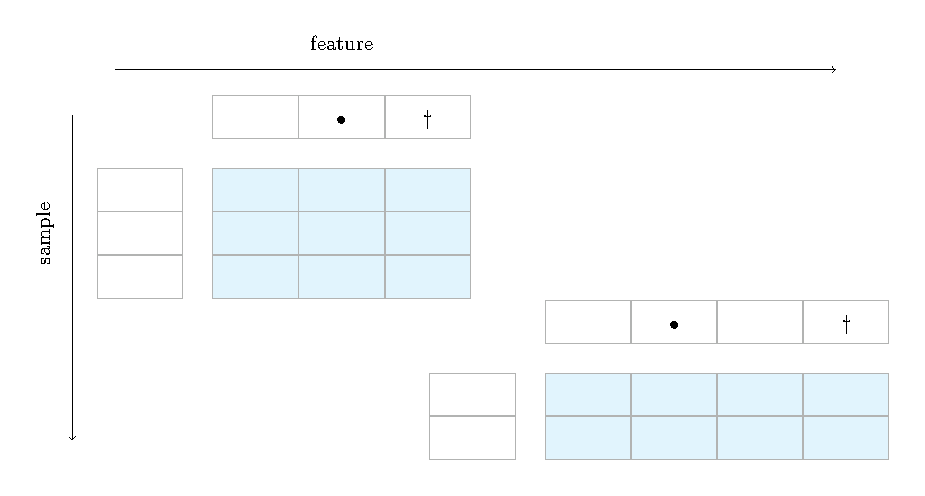
\includegraphics[height=0.35\textheight]{img/anndata} & 
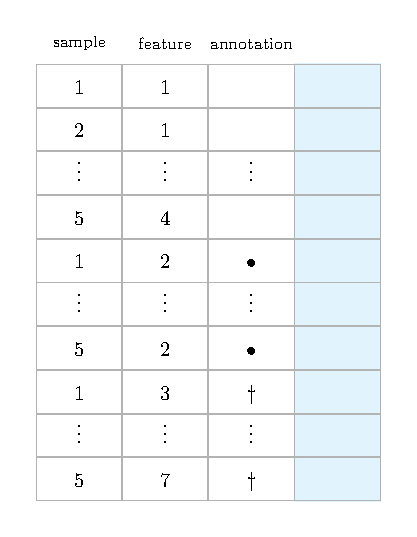
\includegraphics[height=0.35\textheight]{img/ann_tidy}\\
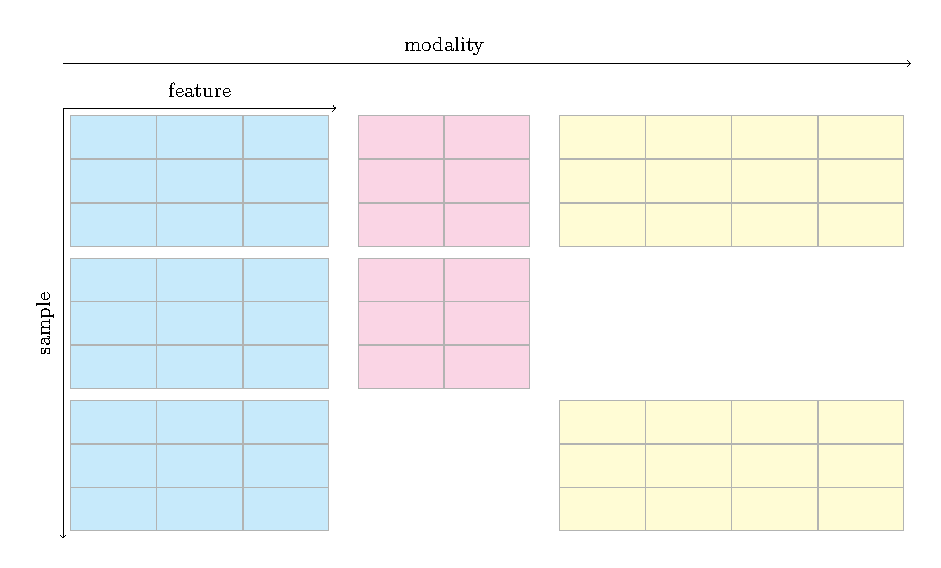
\includegraphics[height=0.35\textheight]{img/mmdata} &
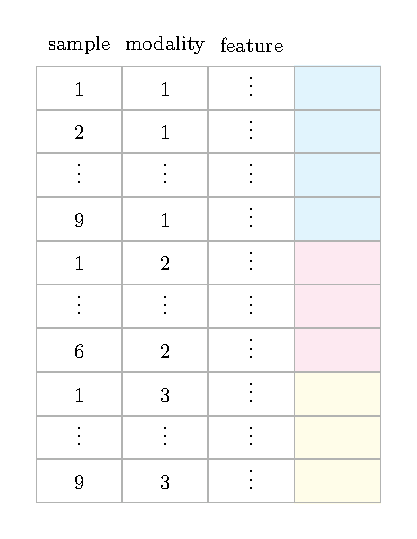
\includegraphics[height=0.35\textheight]{img/mm_tidy}
\end{tabular}
\end{figure}
 tidy-format の利便性を生かしたまま行列分解ができないか?
}
\frame{
\frametitle{例: 3階のテンソルの場合}
Data:
$$
 Y=(y_{ijk}), \quad y=(y_n) = \operatorname{vec}(Y) .
$$

CP分解:
\begin{equation*}
y_{ijk} \approx \sum_{l}v_{il}^{(1)} v_{jl}^{(2)} v_{kl}^{(3)}. 
\end{equation*}

提案法\footnote{Ko ABE and Teppei SHIMAMURA (2023) UNMF: A unified non-negative matrix factorization for multi-dimensional omics data. Briefings in Bioinformatics. \url{https://github.com/abikoushi/moltenNMF}}:
\begin{equation*}
y_{n} \approx \sum_{l}\prod_{d=1}^D v_{dl}^{x_{nd}} \label{eq_approx}
\end{equation*}
ここで, 
\begin{align*}
V=\begin{pmatrix}
V^{(1)}\\
V^{(2)}\\
V^{(3)} 
\end{pmatrix}.
\end{align*}
}
\frame{
\frametitle{内積としての解釈}
\begin{align*}
y_{n}  \approx\sum_{l=1}^L \prod_{d=1}^D v_{dl}^{x_{nd}} &= v_{11}^{x_{n1}} v_{21}^{x_{n2}}\cdots  v_{D1}^{x_{nD}}+ \cdots + v_{1L}^{x_{n1}} v_{2L}^{x_{n2}}\cdots  v_{DL}^{x_{nD}}\\
&=
 \underbrace{
 \color{RedOrange}
\begin{pmatrix}
v_{d1}^{x_{nd}} &  \ldots  & v_{dL}^{x_{nd}}
 \end{pmatrix} 
 \color{RoyalBlue}
 \begin{pmatrix}
\prod _{d' \neq d}v_{d'1}^{x_{nd'}}\\
 \vdots \\
 \prod _{d' \neq d}v_{d'L}^{x_{nd'}}
 \end{pmatrix}
 }_{\mbox{inner product}}
\end{align*}

\begin{figure}
\begin{tabular}{ccc}
inner product of \Huge $($
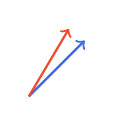
\begin{tikzpicture}
\draw[thick,->,color=RoyalBlue] (0,0)--(0.71,0.71); 
  \draw[thick,->,color=RedOrange] (0,0)--(0.51,0.86);
\end{tikzpicture}
$)$
&
\Large $>$
&
inner product of \Huge $($
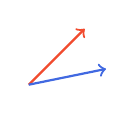
\begin{tikzpicture}
 \draw[thick,->,color=RedOrange] (0,0)--(0.71,0.71);
  \draw[thick,->,color=RoyalBlue] (0,0)--(0.98,0.2);
\end{tikzpicture}
$)$
\end{tabular}
\caption{$y_n$の値が大きいとき$V$の$X$ で指定される成分どうしの値が似る}
\end{figure}
}
\frame{
\frametitle{アンサンブルとしての解釈}
\begin{align*}
y_{n}  \approx\ &\sum_{l=1}^L\prod_{d=1}^D v_{dl}^{x_{nd}} \\
&=\frac{1}{L}\sum_{l=1}^L \underbrace{ L\exp\left( \sum_{d=1}^D x_{nd}  \cdot \log v_{dl}\right) }_{\mbox{log-linear model}}
%&= \frac{1}{L}\sum_{l=1}^L L f_{nl} \quad \mbox{\structure{(mean of the log-linear predictor)}}
\end{align*}
\begin{figure}
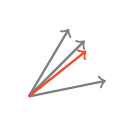
\begin{tikzpicture}
\draw[thick,->,color=gray] (0,0)--(0.71,0.71); 
\draw[thick,->,color=gray] (0,0)--(0.51,0.86);
\draw[thick,->,color=gray](0,0)--(0.98,0.2);
\draw[thick,->,color=RedOrange](0,0)--(0.73,0.58);
\end{tikzpicture}
\caption{複数の対数線形モデルの平均と捉えられる}
\end{figure}
}
\frame{
\frametitle{モデル(準備)}

式1$\left( y_{n} \approx \sum_{l} \prod_{d=1}^D v_{dl}^{x_{nd}}\right)$ より\footnote{cf. Abe \& Shimamura (2023) はポアソン分布を仮定.}
\begin{align}
y_n \mid V, \lambda & \sim \normal\left(y_n \mid \sum_{l=1}^L \prod_{d=1}^D v_{dl}^{x_{nd}}, \lambda^{-1}\right) \label{eq_mod1}\\
v_{dl} & \sim \normal(v_{dl} | 0,\tau^{-1}) \label{eq_prior1}\\
\lambda & \sim \gam(\lambda | a,b) \nonumber
\end{align}
ここで $\normal(x|\mu,\sigma^2)$ は正規分布(平均$\mu$,分散$\sigma^2$) $\gam(x | a,b)$ はガンマ分布(形状パラメータ$a$, レートパラメータ$b$).
\begin{itemize}
\item さらに修正・拡張
\begin{itemize}
\item 解釈性のため:非負制約 
\item マルチオミクスデータの分析のため:分布を変える
\end{itemize}
\end{itemize}
}
\frame{
\frametitle{事前分布:非負制約}
\begin{align*}
v_{dl} & \sim \truncnorm(v_{dl} | 0,\tau^{-1})  \\ \label{eq_prior2}
& \propto \normal(v_{dl} | 0,\tau^{-1})\one_{(0,\infty)}(v_{dl})
\end{align*}
ここで, $\one_{A}(x)$ は指示関数($x \in A$ のとき1,さもなくば0).

\vspace{\baselineskip}

\structure{Note:} 原理的には, 非負制約の有無は変数ごとに選ぶこともできるが, 今回の我々の実装では煩雑さを避けるためすべて非負とした.
}
\frame{
\frametitle{中間変数:分布を変える}
\begin{itemize}
\item $y_n$ が実数(連続値):
$$
A(x)=x.
$$
\item 
$y_n$ が非負:非負化
$$
A(x)=\begin{cases}x, &x>0\\0 &x\leq 0\end{cases}
$$
\item
$y_n$ が2値(0 or 1):2値化
$$
A(x)=\one_{(0,\infty)}(x)
$$
\item
$y_n$ が非負の整数:離散化
$$
A(x)=\begin{cases}\lceil x\rceil, & x>0\\0 &x\leq 0\end{cases}
$$
\end{itemize}
}
\frame{
\frametitle{切断, 非負化, 離散化}
\begin{figure}
\centering
\begin{tabular}{c|cc}
\subfloat[切断]{ 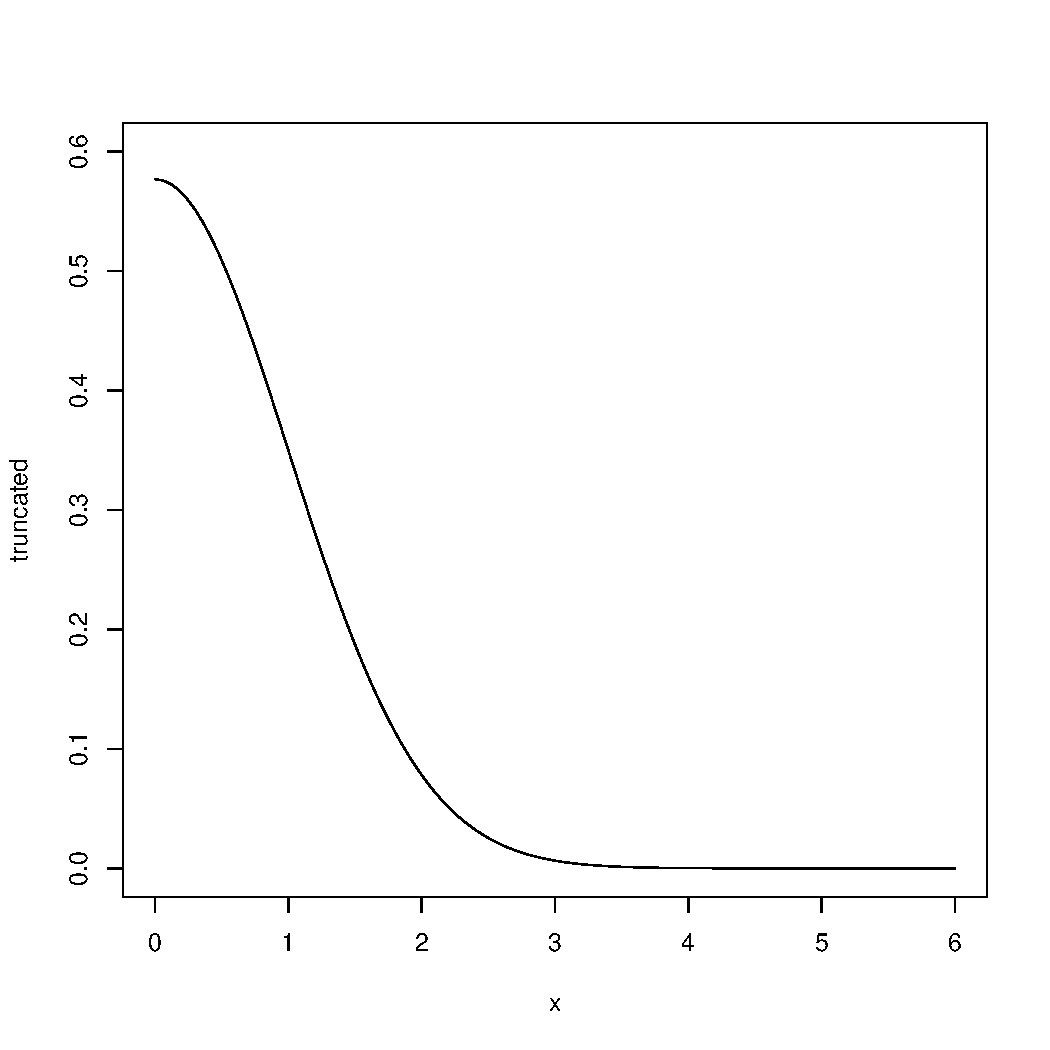
\includegraphics[width=0.3\textwidth]{img/norm_truncated}}&
\subfloat[非負化]{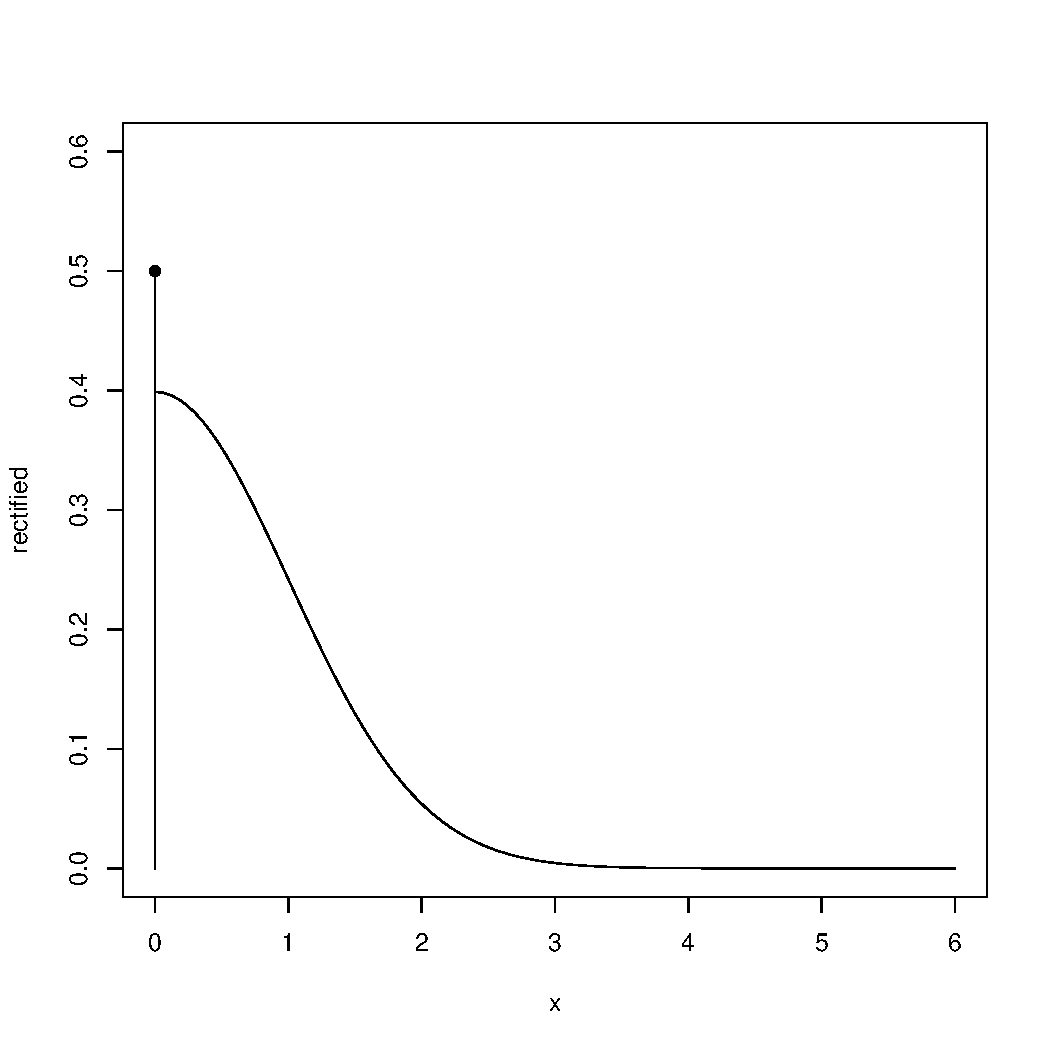
\includegraphics[width=0.3\textwidth]{img/norm_rectified}}&
\subfloat[離散化]{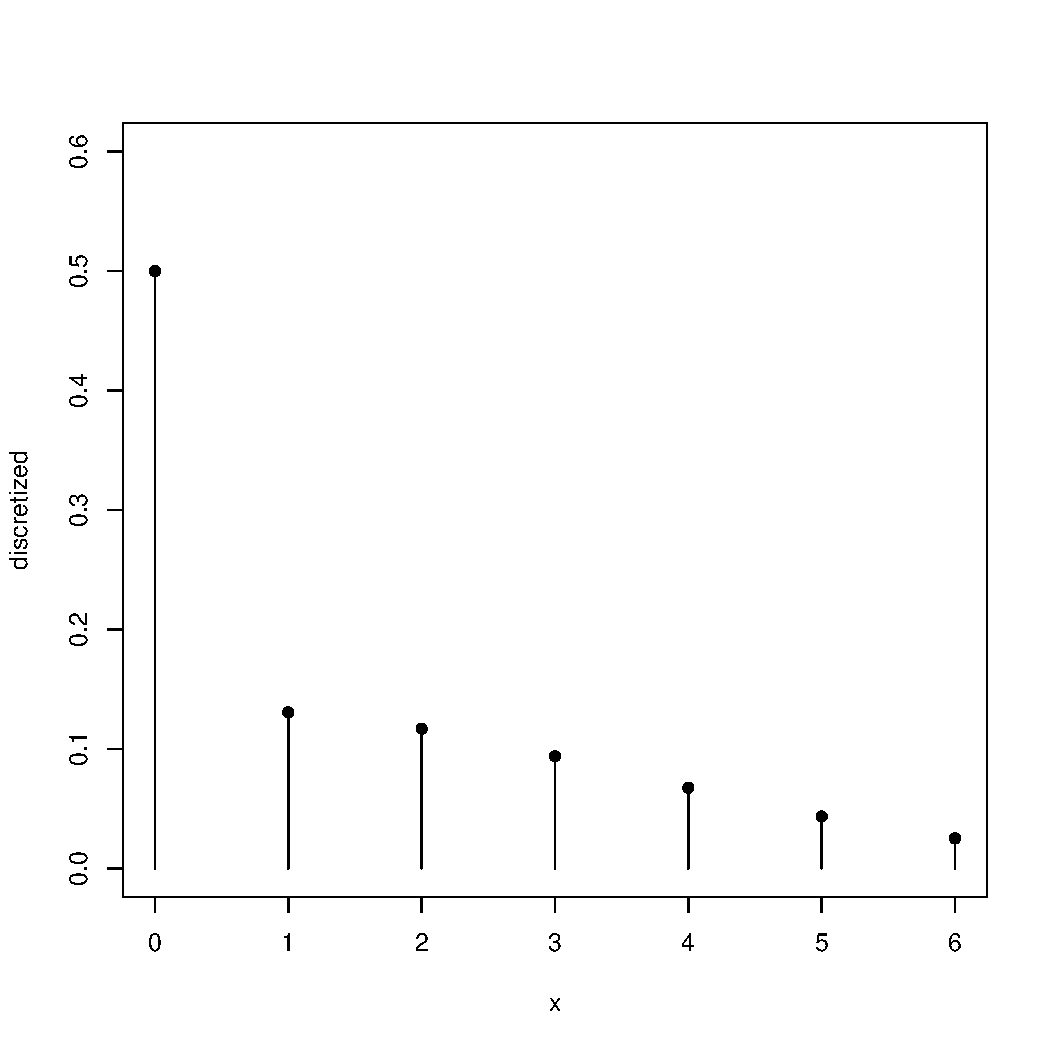
\includegraphics[width=0.3\textwidth]{img/norm_discretized}}
\end{tabular}
\caption{a: 潜在変数の事前分布. b, c: 観測されるデータのモデル. 観測されるデータのモデルは0の一点で確率を持つ(cf. zero-inflated モデル)}
\end{figure}

%\vspace{\baselineskip}

\structure{Note:} モデルの密度が0になることは対数尤度に$-\infty$の罰則をつけることと同じであるため, 分布の台が特に大きい影響を持つと考えた.
}
\frame{
\frametitle{モデル}

\begin{equation}
y_{n} = A_{m(n)}(z_{n}), \quad z_{n} \sim \mathcal{N}\left(\sum_{l=1}^L \prod_{d=1}^Dv_{dl}^{x_{nd}}, \lambda^{-1}\right) \label{eq_mod2}    
\end{equation}
ここで $m(n)$ は $n$ をモダリティを区別する添字に写す関数. 

\vspace{\baselineskip}

分析者が設定する要素(チューニングパラメータ):
\begin{itemize}
\item[] 潜在変数$V$の次元$L$
\item[] 中間的関数$A(x)$
\item[] 計画行列$X$
\end{itemize}
}
\frame{
\frametitle{対数尤度}
\begin{align*}
 \ell(v_{dl}) &=\sum_{n=1}^{N} \log p(z|V, X) = \sum_{n=1}^{N}\left(-\frac{\lambda}{2}\left\{ z_n -\sum_{l=1}^L\prod_{d=1}^D v_{dl}^{x_{nd}} \right\}^2\right)+ \C\\
&= -\frac{h_{dl}}{2}\left(v_{dl}^2-2v_{dl}\frac{\eta_{dl}}{h_{dl}}\right) +C,
\end{align*}
ここで,
\begin{align}
\eta_{dl} &= \sum_n x_{nd} \prod_{d' \neq d} v_{dl}^{x_{nd}}\left( z_{n} - \sum_{l'\neq l} \prod_{d' \neq d} v_{dl}^{x_{nd}} \right) \label{eq_eta}\\
h_{dl} &= \sum_n \lambda x_{nd} \prod_{d' \neq d} v_{dl}^{2x_{nd}}. \label{eq_h}
\end{align}
$v_{dl}$ に依存しない定数をまとめて $C$ とした.
}
\frame{
\frametitle{変分EMアルゴリズム(一般論)}

\begin{itemize}
\item[] データ: $\mathcal{D}=(\mathcal{D}_1,\mathcal{D}_2,\ldots,\mathcal{D}_n)$ 
\item[] $\mathcal{D}$ 全体に影響する \structure{global} な潜在変数: $V$
\item[] $\mathcal{D}_n$ に影響する \structure{local} な潜在変数: $z_n$ ($z=(z_1,\ldots,z_N)'$)
\end{itemize}

\begin{align*}
D_{KL}(q\|p) &=\int q(z) \log \frac{q(z)}{p(z_n|\mathcal{D},w)} dz\\
&= E_q [ \log q(z)] - E_q[\log p(z_n|\mathcal{D},w)]
\end{align*}
$q(z) \propto  \exp( E_q[\log p(z_n|\mathcal{D},w)])$ のとき最小.


\begin{block}{変分EMアルゴリズム}
\begin{itemize}
\item []\structure{ E-step:}  $q(z_n) \propto  \exp( E_q[\log p(z_n|\mathcal{D},w)])$ を更新
\item[] \structure{M-step:}  $q(w) \propto  \exp( E_q[\log p(w|\mathcal{D},z)])$を更新
\end{itemize}
\end{block}
}
\frame{
\frametitle{local な潜在変数(提案モデル)}

変分事後分布からサンプリング:
\begin{itemize}
\item 非負化:
\begin{align}
q(-z_n) = \begin{cases}
    \mathcal{TN}(-z_n|-f_n, \sigma_n^2) & y_n=0,\\
    z_n = y_n \mbox{~with probability 1} & y_n>0
\end{cases} \label{qz_rect}
\end{align}
\item 2値化:
\begin{align}
q(-z_n) = \begin{cases}
    \mathcal{TN}(-z_n|-f_n, \sigma_n^2) & y_n=0,\\
    \mathcal{TN}(z_n|f_n, \sigma_n^2) & y_n=1
\end{cases} \label{qz_binary}
\end{align}
\item 離散化:
\begin{align}
q(-z_n) = \begin{cases}
    \mathcal{TN}(-z_n|-f_n, \sigma_n^2) & y_n=0,\\
    \mathcal{TN}(z_n|f_n, \sigma_n^2) & y_n=1
\end{cases} \label{qz_binary}
\end{align}
\end{itemize}
}
\frame{
\frametitle{globalな潜在変数(提案モデル)}
解析的に期待値計算:
\begin{align}
q(v_{dl})= \begin{cases}
\normal(\mu_{dl}, \sigma_{dl}) & \mbox{if the prior of $v_{dl}$ is not truncated} \\
\truncnorm(\mu_{dl}, \sigma_{dl}) & \mbox{if the prior of $v_{dl}$ is truncated},     
\end{cases} \label{qv}
\end{align}
ここで, 
\begin{align*}
\mu_{dl} &=\frac{E_q[ \eta_{dl} ]}{E_q[ h_{dl}]+\tau/E_q[\lambda]},\\
\sigma^2 &=\left(\tau + E_q[ h_{dl} ] \right)^{-1}.
\end{align*}
$\lambda$ の変分事後分布は,  
\begin{align}
    q(\lambda) = \gam\left((N/2) E_q[ \eta_{dl}], \left(E_q[ h_{dl}] +\tau\right)/2\right). \label{qlam}
\end{align}
%ここでは, 乱数でサンプリングする $z_n$ を特に $\tilde z_n$ と書いた.
}

\begin{frame}[fragile=singleslide]
\frametitle{データ分析}
\begin{itemize}
\item Kostic et al. (2015): ヒト腸内細菌叢と代謝物(メタボローム)のコホート調査. 糖尿病予備軍の乳幼児に関する.
\begin{small}
\begin{verbatim}
R> ~ subject + colname + age + month + CaseControl + modality
\end{verbatim}
\end{small}
\item  GSE146188 : 5種の哺乳類(ヒト, マウス, ブタ, カニクイザル, アカゲザル)の, シングルセル(1細胞ごとの)RNA-seq data.
\end{itemize}
\end{frame}

\frame{
\frametitle{Kostic et al. (2015)}
\begin{figure}
\begin{tabular}{l}
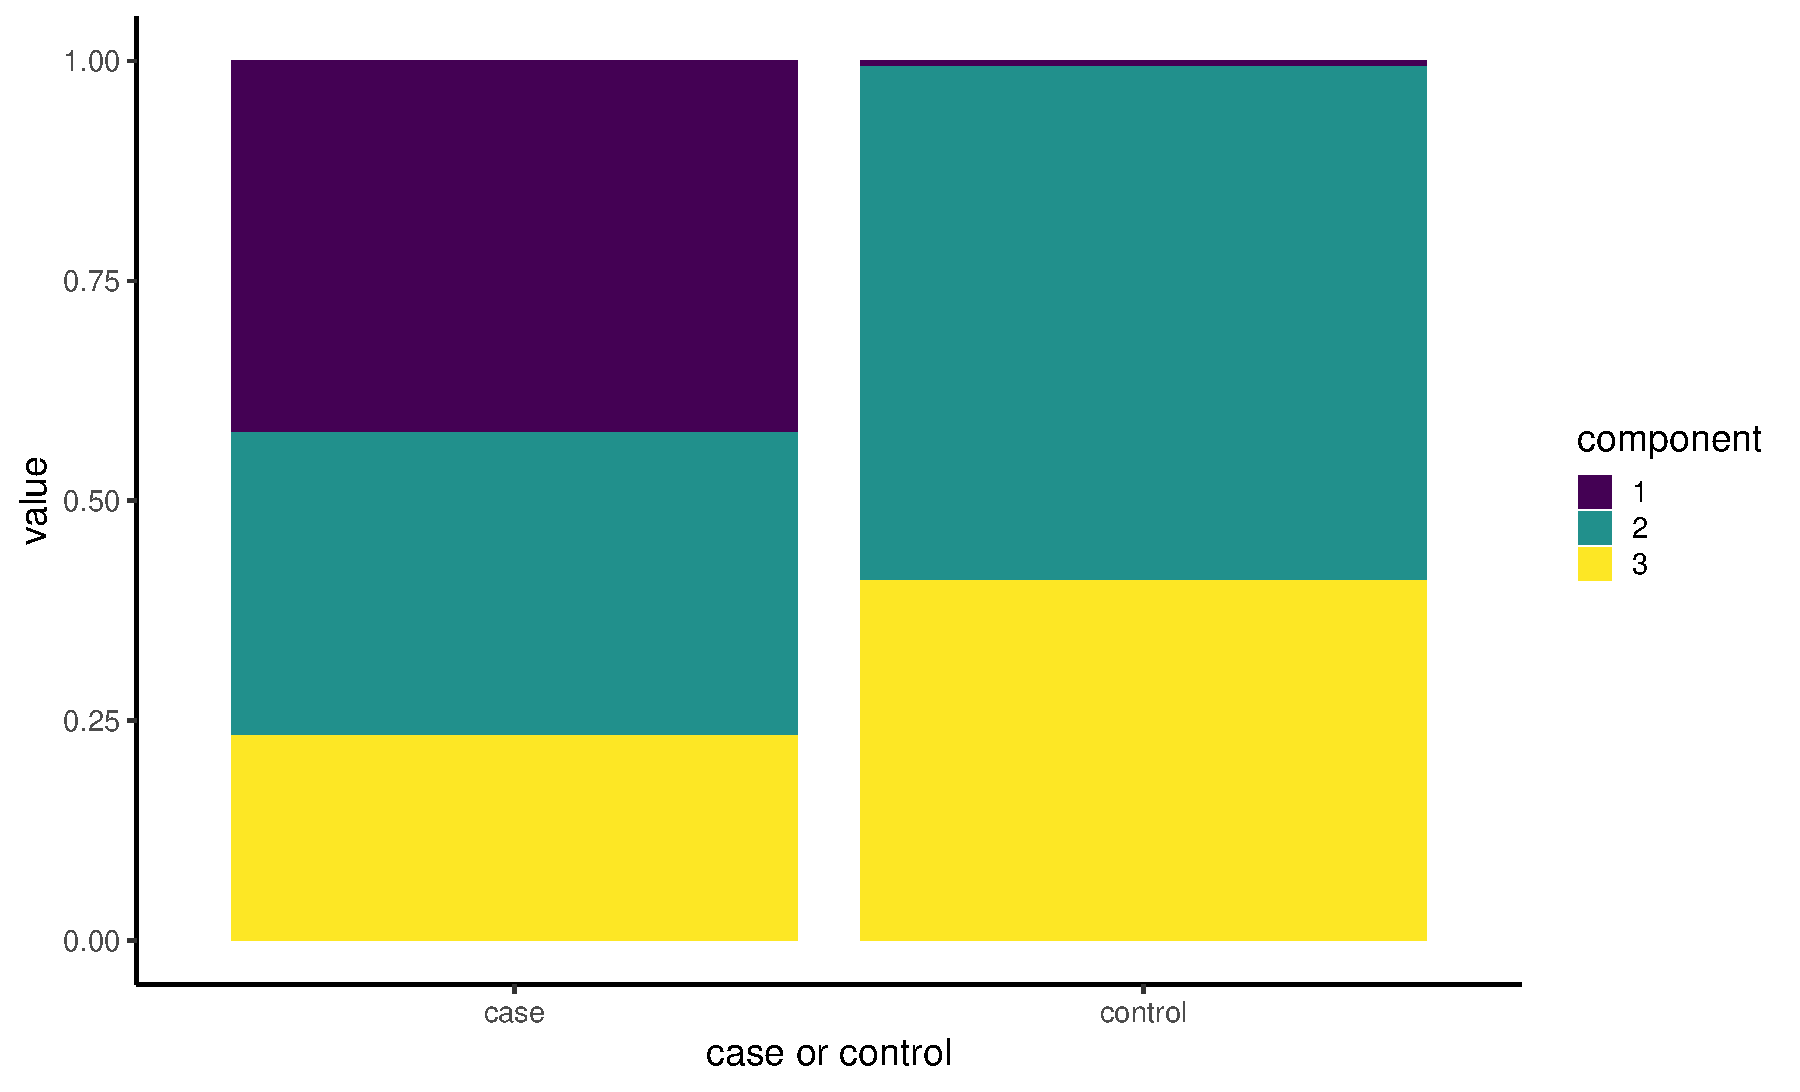
\includegraphics[height=0.3\textheight]{img/Kostic_case.pdf} \\
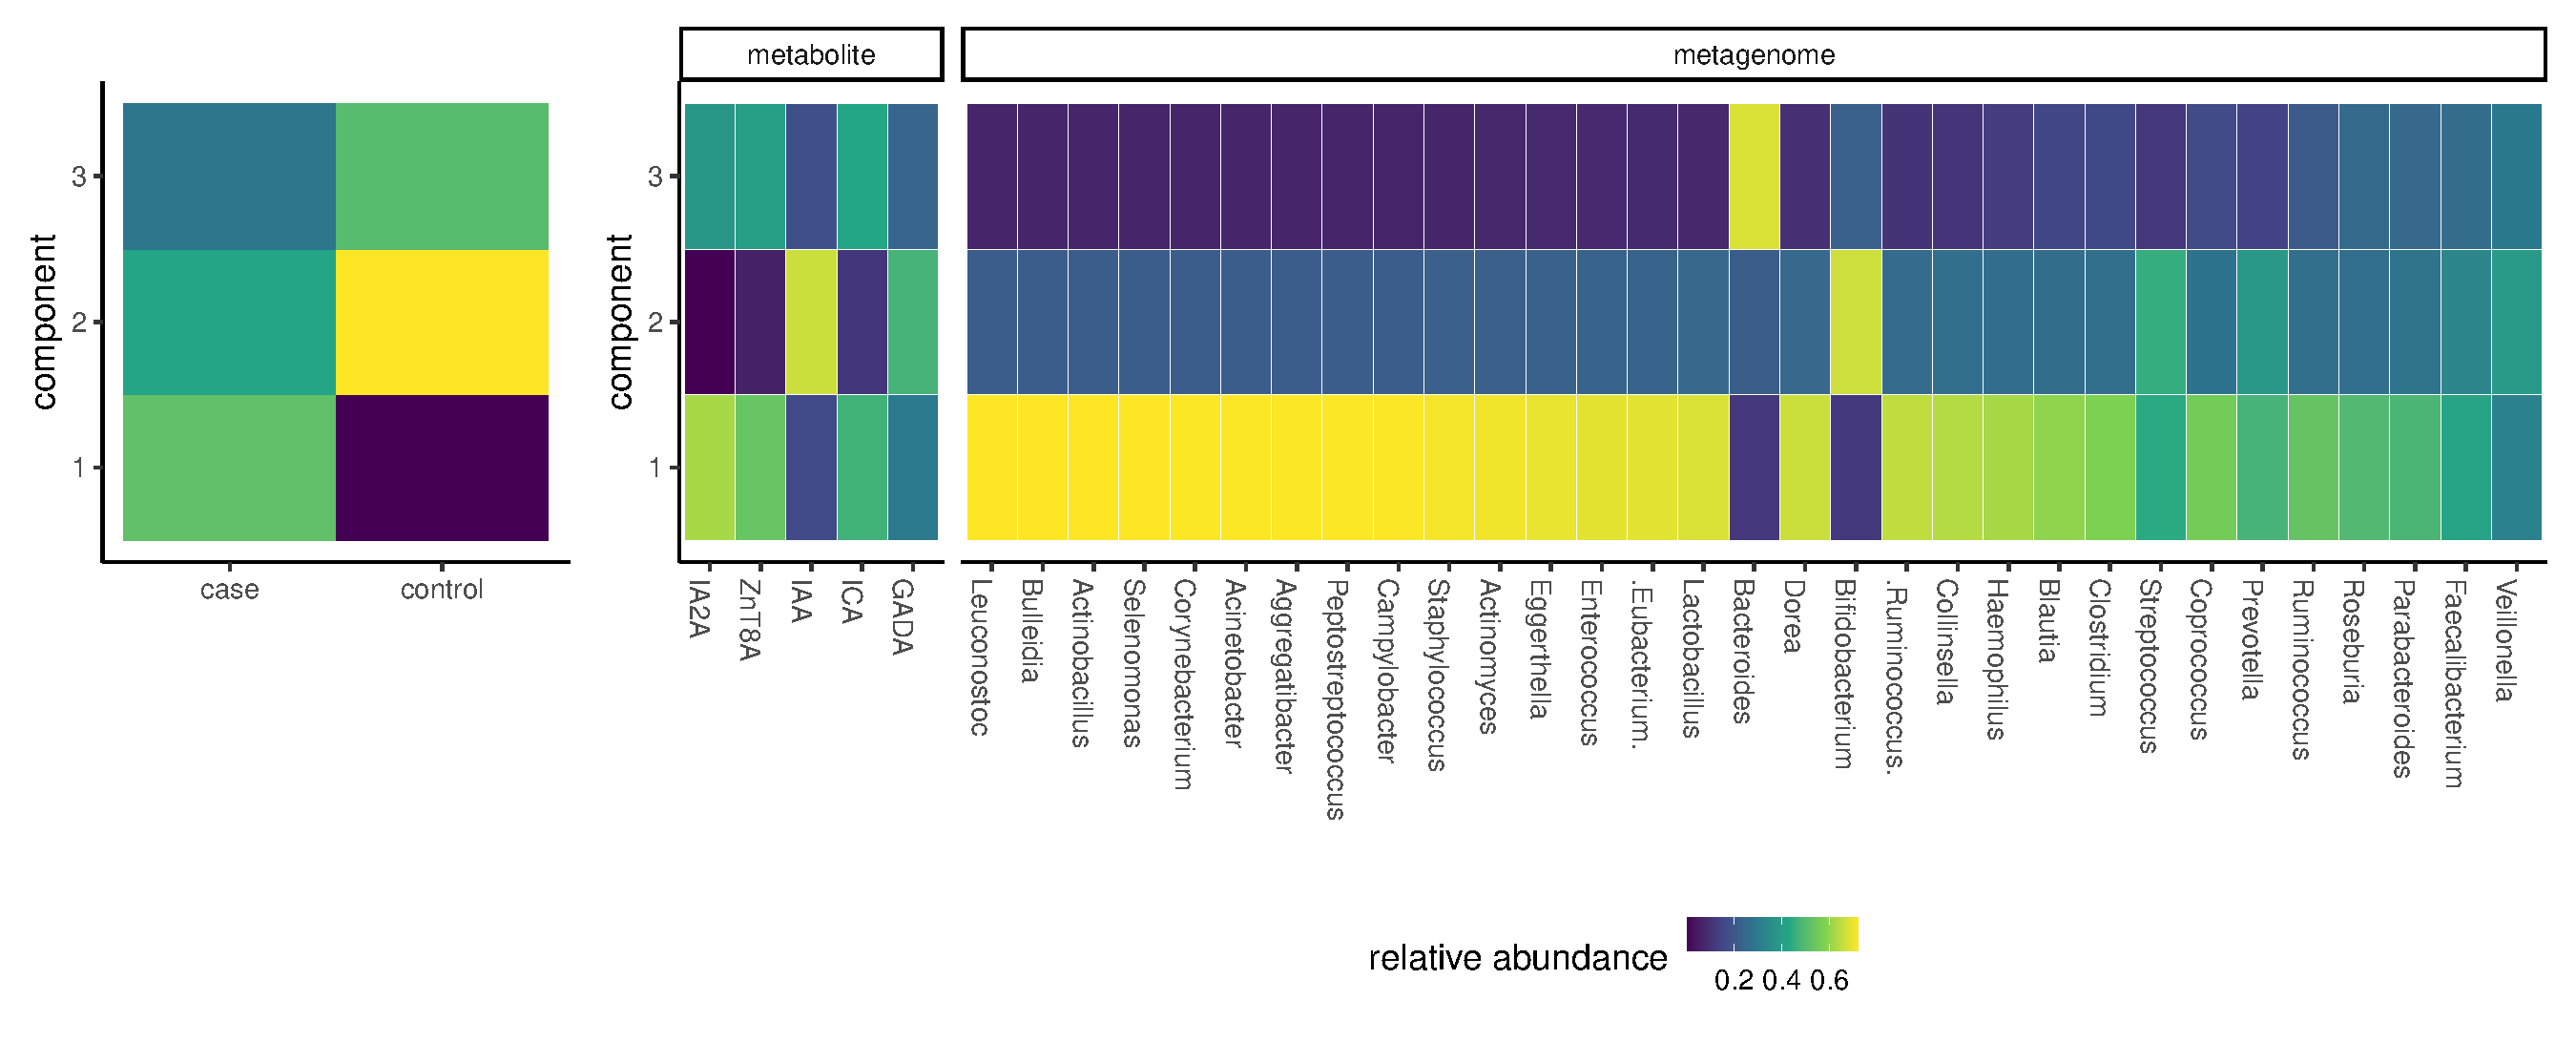
\includegraphics[height=0.45\textheight]{img/Kostic_name.pdf}
\end{tabular}
\caption{component 1 が case(糖尿病)に相対的に豊富な細菌のグループ.}
\end{figure}
}
\frame{
\frametitle{まとめ}

CP分解を特殊な場合として含む統計モデルと, 変分ベイズ法に基づくその推定量を提案した.

\setbeamertemplate{itemize item}{\color{orange}$\blacktriangleright$}
\begin{itemize}
\item 多様なデータに適用できる柔軟性
\item 解釈性
\end{itemize}

\structure{今後の発展:}大規模メタアナリシス, 因果推論, 時空間の相関を考慮
%(学習済みword2vec のようなイメージ)
%(g-formula)
}
\end{document} 